\begin{blocksection}
CALL is an acronym for the process that C source code goes through before being executed by the computer. The four steps are Compiler, Assembler, Linker, and Loader. 
One benefit of using so many stages is that individual parts of a program can be compiled separately before being linked into the final executable. 
This can be very helpful when working with massive programs!

 %\begin{tabular}{ |l|l|l| } 
 %\hline
 %Step & Input & Output \\
 %\hline
 %Compiler & \makecell{C source code (foo.c) \\ #directives have already been handled by the preprocessor before this step} & \makecell{Assembly language (foo.s for RISC-V) \\ Output can contain pseudo instructions like la, nop, li, mv, j, etc.} \\
 %\hline
 %Assembler & \makecell{Assembly language (foo.s)} & \makecell{Object file containing object code & information tables (foo.o for RISC-V) \\ \\ Directives (.text, .word, .data, etc.) which specify formatting without producing any machine code are interpreted and pseudo instructions are replaced. Symbol table, which lists functions and variables that can be called by other files, and relocation table, which tracks labels and data within the code that still needs to be filled in, are created.} \\
 %\hline
 %Linker & \makecell{One or more object files (foo.o, lib.o, stuff.o) \\ \\ Each object file can be compiled up to this point independently, so an update to a library or a refactoring of code does not require recompilation of everything.} & \makecell{Executable (a.out) \\ The text segments from each file are concatenated together and the data segments likewise. The reference tables are resolved as the linker has access to the final text/data section and can calculate absolute addresses/offsets.} \\
 %\hline
 %Loader & \makecell{Executable (a.out) \\ Handled by the OS} & \makecell{Program execution by computer \\ \\ Header is read and instructions/data from the executable are copied into a newly allocated address space}
 %end{tabular}
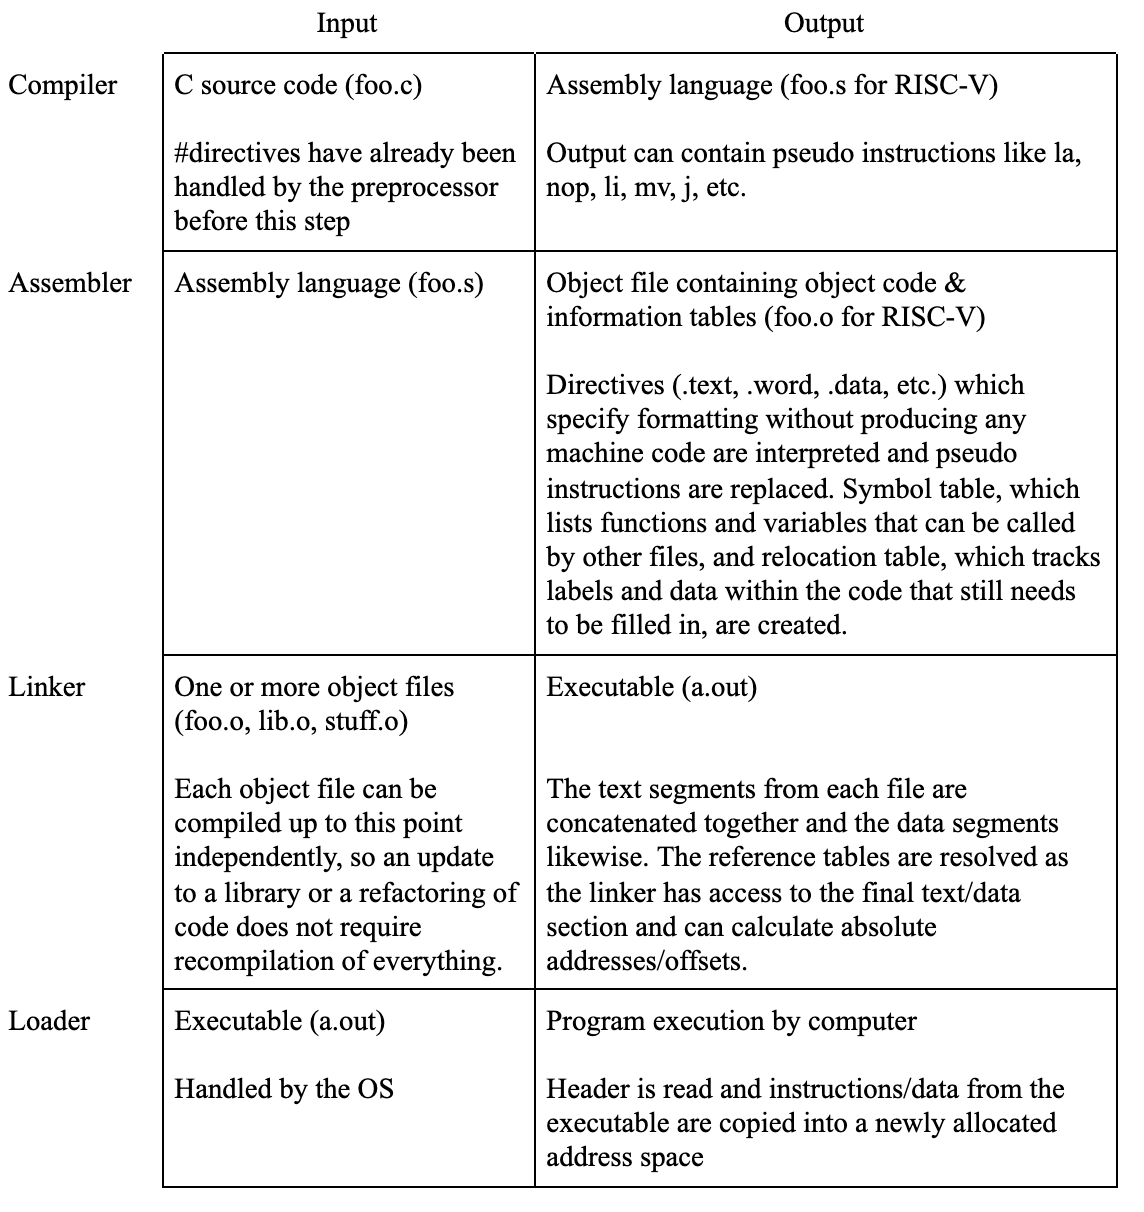
\includegraphics[width=\textwidth]{images/call/table.png}

\end{blocksection}